\section{Results}
\label{sec:evaluation}
We present the results following the four research questions. RQ1 maps where planning beats direct execution as the register grows, including beyond device memory. RQ2 repeats the comparison for gradient workloads and inside training loops. RQ3 measures how good the planner's decisions are and how much it pays to make them, and RQ4 collects the mechanisms that do not pay off. All simulated results passed validation: no value differed from its reference by more than $10^{-9}$. Hardware estimates are compared with exact values in Section~\ref{sec:rq4}.

\subsection{RQ1: Where does planning beat direct execution?}
\label{sec:rq1}
\begin{figure*}[!t]
\centering
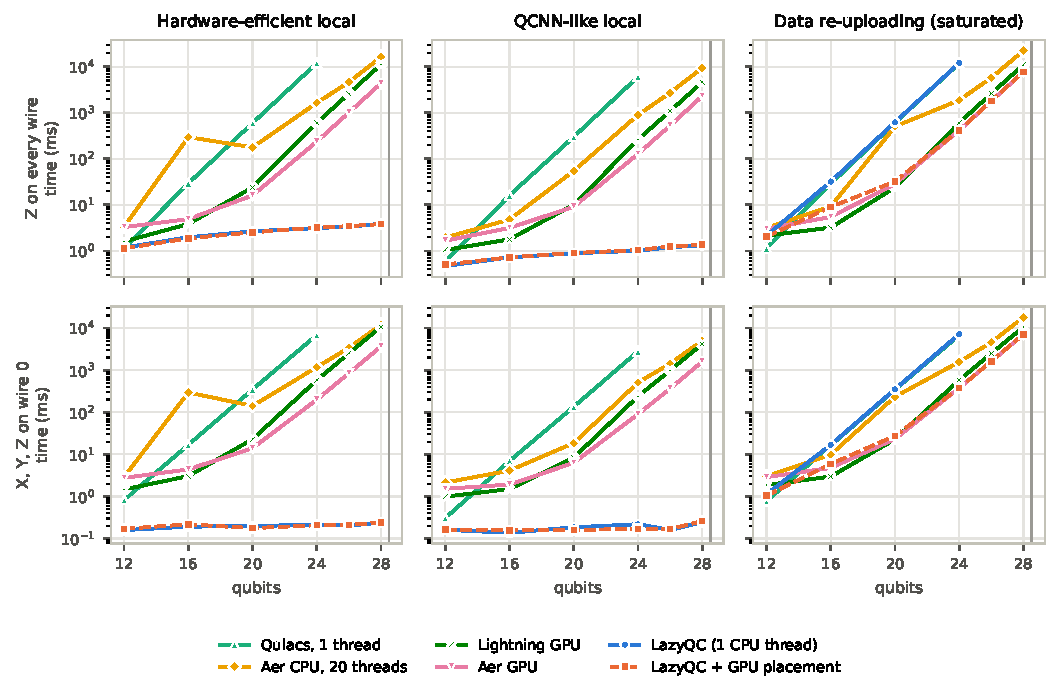
\includegraphics[width=\textwidth]{figures/direct_scaling.pdf}
\caption{Time to obtain every requested expectation value as the register grows, for the three circuit families (columns) and the two output patterns (rows). Each point is the median over repetitions of one case, averaged geometrically over two held-out seeds. The planner runs on one CPU thread and is charged with its analysis; direct methods receive prebuilt circuits and all 20 host threads. The vertical line marks the 28-qubit limit of the 8\,GB GPU in double precision. Aer CPU is slower at 16 than at 20 qubits on the hardware-efficient family, where synchronizing 20 threads dominates the small state. Lower is better.}
\label{fig:direct-scaling}
\end{figure*}

\begin{table}[!t]
\caption{Fastest Direct Method's Time Divided by the Planner's Time, with GPU Placement Enabled, by Number of Qubits. Values Above One Favour the Planner.}
\label{tab:rq1}
\centering
\setlength{\tabcolsep}{3pt}
\footnotesize
\resizebox{\columnwidth}{!}{\begin{tabular}{llrrrrrr}
\toprule
Family & Outputs & 12 & 16 & 20 & 24 & 26 & 28\\
\midrule
Hardware-eff. & $Z$, all & 1.00 & 2.05 & 6.34 & 73.3 & 295 & 1{,}137\\
Hardware-eff. & $X,Y,Z$, one & 4.84 & 14.0 & 79.5 & 960 & 3{,}987 & 15{,}279\\
QCNN-like & $Z$, all & 1.15 & 2.46 & 10.2 & 122 & 424 & 1{,}681\\
QCNN-like & $X,Y,Z$, one & 1.87 & 9.55 & 39.6 & 529 & 2{,}177 & 6{,}111\\
Re-uploading & $Z$, all & 0.56 & 0.36 & 0.74 & 1.00 & 1.00 & 1.00\\
Re-uploading & $X,Y,Z$, one & 0.74 & 0.50 & 0.83 & 1.01 & 1.00 & 1.00\\
\bottomrule
\end{tabular}
}
\end{table}

Fig.~\ref{fig:direct-scaling} shows the time needed to obtain every requested output as the register grows from 12 to 28 qubits, and Table~\ref{tab:rq1} gives the ratio between the fastest direct method and the planner. Three regimes stand out.

\textbf{Local families: work that no device can avoid.} For the hardware-efficient and QCNN-like families, the planner's time is almost flat. With $Z$ on every wire, it grows from 1.1 to 3.8\,ms (hardware-efficient) and from 0.5 to 1.4\,ms (QCNN-like) between 12 and 28 qubits, because every output keeps a cone of at most 10 and 8 qubits respectively, while every direct method doubles its cost with each added qubit. At 28 qubits the planner groups the 28 outputs of the hardware-efficient circuit into 14 tasks of at most 10 qubits and spends 1.4\,ms planning and 2.3\,ms collecting them, whereas the fastest direct method, Aer on the GPU, needs 4.35\,s. On a single CPU thread the planner ties with single-thread Qulacs at 12 qubits, and is 2.0 to 2.5 times faster than the fastest GPU method at 16 qubits (1.6 to 2.2 times in a later confirmation run), 6 to 10 times at 20, 73 to 122 times at 24 and 1,137 to 1,681 times at 28. When only the three Paulis on one wire are requested, a dense state serves fewer outputs and the margins grow further, from 1.9 to 4.8 times at 12 qubits to 6,111 to 15,279 times at 28. These ratios are large because the direct curves grow exponentially while the planner's do not. They are specific to our laptop GPU, but a faster GPU moves the direct curves down by a constant factor without changing their slope (Section~\ref{sec:discussion}).

\textbf{Saturated cones: hand the work over.} In the data re-uploading family every cone spans the whole register and the planner keeps the dense plan. On one CPU thread this costs what single-thread Qulacs costs plus the planner's overhead, which is visible at small widths (2.1 against 1.1\,ms at 12 qubits) and negligible at large ones (12.1 against 11.9\,s at 24 qubits). With width-based placement the dense task runs on the GPU instead. The fixed costs of planning, lowering the circuit and launching it make the planner 0.36 to 0.83 times as fast as the fastest GPU method between 16 and 20 qubits, but from 24 qubits on it matches direct Aer GPU within 0.6\% (0.997 to 1.006 times). The planner cannot speed up saturated work, but it does not need to make it slower either.

\textbf{Small circuits.} At 12 qubits every method takes about a millisecond and fixed costs dominate the comparison. The planner pays up to 0.6\,ms of analysis and 0.4\,ms of circuit lowering that direct methods with prebuilt circuits do not pay. It is still 1.15 to 4.8 times faster than the best direct method on three of the four local configurations, ties on the fourth and is 0.56 to 0.74 times as fast on the saturated control. The analysis budget of Section~\ref{sec:system} only skips analysis that could not pay even if every cone were free, so it rarely triggers at these sizes; RQ3 examines its effect on the cost of deciding.

\begin{table}[!t]
\caption{Held-Out Families on One CPU Thread: Planner Time over Direct Qulacs and Cross-Validated Selection Regret, Medians per Stratum at One Collection. The Five Top Strata Are Disjoint and Sum to 480; the Width Rows Break Down Their 405-Case Saturated Subset and Are Not Added Again. F, S and G Count the Full, Separate and Grouped Plans Chosen by \texttt{auto}.}
\label{tab:heldout}
\centering
\setlength{\tabcolsep}{3pt}
\footnotesize
\resizebox{\columnwidth}{!}{\begin{tabular}{lrlrr}
\toprule
Stratum & Cases & Auto choice & Auto/direct & CV regret\\
\midrule
\multicolumn{5}{l}{\emph{Disjoint family/cone strata (480 cases)}}\\
Tree, narrow, shared & 15 & G\,15 & 0.016 & 1.14\\
Tree, narrow, distinct & 10 & S\,10 & 0.003 & 1.07\\
Tree, intermediate & 50 & S\,35, G\,15 & 0.29 & 1.05\\
Tree, saturated & 165 & F\,100, G\,55, S\,10 & 1.12 & 1.06\\
Strongly ent., saturated & 240 & F\,170, G\,70 & 1.07 & 1.04\\
\midrule
\multicolumn{5}{l}{\emph{Width breakdown of the 405 saturated cases (overlapping rows)}}\\
Saturated, 8 qubits & 105 & F\,75, G\,30 & 1.82 & 1.41\\
Saturated, 12 qubits & 105 & F\,70, G\,35 & 1.24 & 1.13\\
Saturated, 16 qubits & 105 & F\,70, G\,30, S\,5 & 1.04 & 1.03\\
Saturated, 20 qubits & 90 & F\,55, G\,30, S\,5 & 1.00 & 1.00\\
\midrule
\multicolumn{5}{l}{\emph{All 480 cases (each counted once)}}\\
All held-out cases & 480 & F\,270, G\,155, S\,55 & 1.07 & 1.05\\
\bottomrule
\end{tabular}
}
\end{table}

\textbf{Unseen families.} The same regimes appear on the two families added after the planner was frozen (Table~\ref{tab:heldout}), here against direct single-thread Qulacs at depths 2 to 16. Where tree cones are narrow and outputs share them, the planner needs 0.016 times the direct time, about 60 times less. With narrow cones that outputs do not share it needs 0.003 times, and with intermediate cones 0.29 times. Where cones saturate, \texttt{auto} keeps the dense plan in two thirds of the cases and pays 1.07 to 1.12 times direct execution. That overhead is a matter of size rather than family: 1.82 times at 8 qubits, where a direct evolution takes 0.2\,ms, 1.24 at 12, 1.04 at 16 and 1.00 at 20. The fixed cost of deciding is visible only while the simulation itself takes about a millisecond.

\begin{table}[!t]
\caption{Same-Backend Comparison with $Z$ on Every Wire: Direct Execution Time Divided by the Time of LazyQC Running Its Tasks on the Same Backend, by Number of Qubits. Values Above One Favour LazyQC. Qulacs Uses One Thread; LazyQC on quimb Uses the Grouped Cone Plan. The quimb Row Is the Legacy Per-Output Comparator; Stronger Shared Tensor-Network Baselines Appear Below.}
\label{tab:backends}
\centering
\setlength{\tabcolsep}{3pt}
\footnotesize
\begin{tabular}{llrrrrr}
\toprule
Backend & Family & 12 & 16 & 20 & 24 & 28\\
\midrule
Qulacs, 1 thread & Hardware-eff. & 0.96 & 14.9 & 226 & 3{,}825 & n/a\\
Qulacs, 1 thread & QCNN-like & 1.24 & 22.3 & 339 & 6{,}030 & n/a\\
Qulacs, 1 thread & Re-uploading & 0.53 & 0.90 & 0.98 & 0.98 & n/a\\
Aer GPU & Hardware-eff. & 0.28 & 0.31 & 0.82 & 9.86 & 149\\
Aer GPU & QCNN-like & 0.19 & 0.26 & 0.71 & 6.76 & 95.8\\
Aer GPU & Re-uploading & 0.66 & 0.73 & 0.96 & 1.01 & 0.98\\
Lightning GPU & Hardware-eff. & 0.22 & 0.39 & 1.88 & 40.1 & 613\\
Lightning GPU & QCNN-like & 0.29 & 0.33 & 1.54 & 33.1 & 503\\
Lightning GPU & Re-uploading & 0.71 & 0.63 & 0.91 & 1.00 & 0.98\\
quimb & Hardware-eff. & 0.96 & 1.06 & 1.46 & 1.05 & 1.06\\
quimb & QCNN-like & 0.92 & 0.92 & 0.94 & 0.95 & 1.00\\
quimb & Re-uploading & 0.84 & 0.84 & 0.84 & 0.90 & 0.80\\
\bottomrule
\end{tabular}

\end{table}

\textbf{Planning on every backend.} The comparison above mixes two choices: whether to plan, and which device to use. To separate them, we ran the planner's tasks on each backend and compared them with direct execution on that same backend (Table~\ref{tab:backends}, 1,440 additional validated timings). On state-vector backends the benefit of planning grows exponentially with the register whatever the device: at 28 qubits, LazyQC on Aer GPU is 96 to 149 times faster than direct Aer GPU, and LazyQC on Lightning GPU 503 to 613 times faster than direct Lightning GPU. Below about 20 qubits, however, sending every small cone task to a GPU is slower than direct execution (0.19 to 0.39 times at 12 and 16 qubits), because each task pays the GPU's fixed launch cost. This is the regime in which width-based placement keeps them on the CPU, and a faster GPU makes it more important, not less: on the H100, LazyQC with every task on the GPU overtakes direct execution only at 28 qubits on Aer (1.8 to 3.0 times) and from 24 qubits on Lightning (2.0 to 2.5 times), whereas with narrow tasks kept on the CPU it wins from 16 qubits. With the legacy per-output quimb workflow, planning gains little (0.92 to 1.46 times with $Z$ on every wire, up to 2.4 times when several outputs share a wire). This row isolates reuse on one implementation; it is not evidence that tensor networks are generally slower, which the shared baselines below directly test. Across all configurations, LazyQC on single-thread Qulacs was the fastest way to evaluate the local families at every width (0.1 to 3.9\,ms), tying with direct Qulacs at 12 qubits on one of them. For the saturated family the best choice moved from Lightning GPU at 16 qubits (about 3\,ms) to quimb at 28 qubits, which evaluated all outputs in 4.4\,s against 7.8\,s for Aer GPU, and three outputs on one wire in 0.15 to 0.20\,s against 7.2\,s.

\begin{table*}[!t]
\caption{Total Batch Time in Milliseconds Beyond Device Memory, Geometric Means over Two Held-Out Seeds. For LazyQC, Width Is the Range of Reduced-Circuit Widths, Not the Logical Register Width $n$ Shown in the Column Headings. Exact MPS Includes Preparation with \texttt{cutoff}${}=0$ and Every Output; $\chi$ Is Its Maximum Bond Dimension. The Saturated Family Has No LazyQC Row Because the Planner Refuses It. Exact MPS Runs Have Three Repetitions and LazyQC Runs Five.}
\label{tab:memory-wall}
\centering
\setlength{\tabcolsep}{3pt}
\footnotesize
\resizebox{\textwidth}{!}{\begin{tabular}{lllrrrrrr}
\toprule
Method & Family & Outputs & Width / $\chi$ & 32 & 48 & 64 & 100 & 128\\
\midrule
LazyQC & Hardware-eff. & $Z$, all & 6--10 & 4.56 & 8.28 & 12.41 & 24.08 & 36.84\\
LazyQC & Hardware-eff. & $X,Y,Z$, one & 6 & 0.24 & 0.26 & 0.30 & 0.42 & 0.48\\
LazyQC & QCNN-like & $Z$, all & 2--8 & 1.65 & 2.53 & 4.00 & 8.11 & 12.64\\
LazyQC & QCNN-like & $X,Y,Z$, one & 8 & 0.20 & 0.19 & 0.21 & 0.27 & 0.27\\
\midrule
Exact MPS & Hardware-eff. & $Z$, all & $\chi{\le}32$ & 67.9 & 106.9 & 142.7 & 228.5 & 273.9\\
Exact MPS & QCNN-like & $Z$, all & $\chi{\le}8$ & 53.0 & 89.1 & 106.1 & 164.4 & 217.4\\
Exact MPS & Re-uploading & $Z$, all & $\chi{\le}16$ & 46.0 & 75.9 & 92.0 & 145.0 & 200.7\\
\midrule
\multicolumn{4}{l}{Dense state (bytes)} & $2^{36}$ & $2^{52}$ & $2^{68}$ & $2^{104}$ & $2^{132}$\\
\bottomrule
\end{tabular}
}
\end{table*}

\textbf{Beyond device memory: narrow cones versus a shared exact MPS.} Direct dense simulation stops at 28 qubits on our GPU, and at 32 qubits it would already need 64\,GiB. Table~\ref{tab:memory-wall} reports both logical width and the widths actually simulated. At 128 qubits with $Z$ on every wire, LazyQC takes 36.84\,ms for the hardware-efficient family, running 64 tasks of width 6--10, and 12.64\,ms for the QCNN-like family, running 112 tasks of width 2--8; planning accounts for 22.99 and 9.34\,ms respectively. With three outputs on one wire it stays below 0.5\,ms. All 44 planned cases in the expanded memory-wall study agree with quimb within $8.3\times10^{-14}$.

The exact global MPS is a much stronger baseline than independent per-output contractions. At 128 qubits it evaluates the same hardware-efficient and QCNN-like batches in 273.93 and 217.44\,ms, so LazyQC retains factors of 7.4 and 17.2 rather than the orders of magnitude suggested by a weak per-output comparison. Its maximum bond dimensions are 32 and 8. For the saturated data-re-uploading family, however, LazyQC refuses every case because no state-vector candidate satisfies the payload limit, whereas exact MPS succeeds: the 48-qubit depth-four batch takes 75.9\,ms and the 128-qubit batch 200.7\,ms. LazyQC's 20 refusals take 0.2 to 55\,ms. Thus the large-width claim is explicitly conditional: narrow-cone planning is faster on these local families; it is not dense 128-qubit simulation, and it is not a replacement for tensor contraction when cones saturate.

\begin{table}[!t]
\caption{Intermediate-Cone Hardware-Efficient Batches at 48 Logical Qubits, with $Z$ on Every Wire. All Entries Include Preparation or Planning and Every Output. The 24 Cone Tasks Have the Width Ranges Shown; a Full 48-Qubit Dense State Does Not Fit on the GPU. Times Are Geometric Means over Two Seeds, in Seconds.}
\label{tab:intermediate-cones}
\centering
\setlength{\tabcolsep}{3pt}
\footnotesize
\resizebox{\columnwidth}{!}{\begin{tabular}{llrr}
\toprule
Method & Width / $\chi$, $d=6/8$ & $d=6$ (s) & $d=8$ (s)\\
\midrule
LazyQC, CPU & 8--14 / 10--18 & 0.073 & 1.476\\
LazyQC, GPU placement & 8--14 / 10--18 & 0.074 & 0.171\\
Exact MPS & $\chi\leq128$ / $\chi\leq512$ & 0.275 & 5.578\\
quimb light-cone TN & -- & 3.270 & 5.566\\
\bottomrule
\end{tabular}
}
\end{table}

\textbf{The intermediate-cone boundary.} Table~\ref{tab:intermediate-cones} fills the missing regime around $w^\star$, reaching $w^\star<w\le28<n$ at depth eight. At depth six, cone widths are 8--14: LazyQC takes about 74\,ms on either placement, against 275\,ms for exact MPS and 3.27\,s for reused-circuit quimb contraction. At depth eight, widths grow to 10--18. CPU-only LazyQC takes 1.476\,s, while routing tasks at or above $w^\star=14$ to the GPU reduces the total to 171\,ms. Exact MPS and reused light-cone contraction take 5.578 and 5.566\,s. In this measured regime, placement contributes an 8.6-fold improvement over CPU-only cone execution, and the complete plan is 32.6 times faster than exact MPS. The result does not define a universal representation crossover: it uses one family at 48 qubits, but it demonstrates why plan selection and device placement must be evaluated separately.

\subsection{RQ2: Gradients and training}
\label{sec:gradients}
\begin{figure*}[!t]
\centering
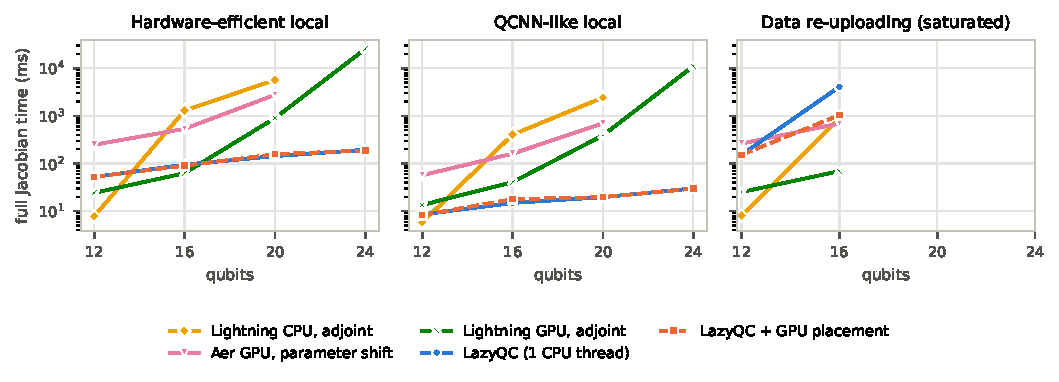
\includegraphics[width=\textwidth]{figures/gradient_scaling.pdf}
\caption{Time to obtain the full Jacobian of all $n$ outputs with respect to every trainable rotation, median per case and geometric mean over two seeds. The planner evaluates the base program and every $\pm\pi/2$ shift as one batch; Aer GPU runs every shifted circuit; Lightning uses adjoint differentiation. At 24 qubits the adjoint Jacobian with all observables exceeded GPU memory and was computed in chunks of eight observables. The saturated family was evaluated up to 16 qubits. Lower is better.}
\label{fig:gradients}
\end{figure*}

\begin{table*}[!t]
\caption{Full Jacobians: Trainable Rotations $P$, Distinct Tasks of the Planner, Structurally Zero Derivatives, and Median Time in Milliseconds per Method.}
\label{tab:jacobian}
\centering
\footnotesize
\setlength{\tabcolsep}{4pt}
\begin{tabular}{lrrrrrrrr}
\toprule
Family & $n$ & $P$ & Tasks & Zeros (\%) & LazyQC & Aer shift & L.\ GPU adj. & L.\ CPU adj.\\
\midrule
Re-uploading & 12 & 48 & 97 & 10 & 152 & 263 & 25 & 8.0\\
Re-uploading & 16 & 64 & 129 & 10 & 1{,}039 & 694 & 69 & 909\\
Hardware-eff. & 12 & 48 & 290 & 51 & 53 & 247 & 24 & 7.8\\
Hardware-eff. & 16 & 64 & 404 & 61 & 90 & 535 & 63 & 1{,}290\\
Hardware-eff. & 20 & 80 & 518 & 68 & 157 & 2{,}761 & 896 & 5{,}656\\
Hardware-eff. & 24 & 96 & 632 & 73 & 187 & n/a & 25{,}310 & n/a\\
QCNN-like & 12 & 22 & 102 & 74 & 8.3 & 57 & 13 & 5.8\\
QCNN-like & 16 & 32 & 158 & 80 & 18 & 161 & 41 & 403\\
QCNN-like & 20 & 38 & 181 & 84 & 20 & 701 & 390 & 2{,}422\\
QCNN-like & 24 & 48 & 237 & 86 & 30 & n/a & 11{,}048 & n/a\\
\bottomrule
\end{tabular}

\end{table*}

Gradient workloads multiply the number of requested circuits. Under the parameter-shift rule of Eq.~\eqref{eq:shift}, one Jacobian with respect to $P$ rotation occurrences requires the base circuit and $2P$ shifted ones, each with all $K$ outputs. They are also where a simulator has its strongest alternative: adjoint differentiation obtains all derivatives of an observable from about two passes over the state~\cite{jones2020adjoint}. We therefore compare the planner's shift-rule Jacobian with Aer GPU running every shifted circuit and with Lightning's adjoint method on the GPU and on the CPU (Fig.~\ref{fig:gradients} and Table~\ref{tab:jacobian}).

The object in this subsection is explicit: a full $K\times P$ Jacobian, with $K=n$ outputs and $(2P+1)K$ raw expectation requests. Table~\ref{tab:jacobian} reports $P$, the planner's distinct tasks, structurally zero entries and absolute times; Fig.~\ref{fig:gradients} compares methods computing that same object. Full Jacobians are useful for multi-output sensitivity, kernel construction and higher-order training methods, but are not required for an ordinary scalar-loss gradient step. The adjoint baseline is therefore configured to return the full Jacobian, including observable chunking when memory requires it; the cheaper scalar-loss vector-Jacobian product is evaluated separately below. The per-request Qiskit LightCone baseline for the raw expectation batch is reported in Table~\ref{tab:lightcone-ablation}.

\textbf{Shift rules meet cones.} The planner receives the $(2P+1)K$ requests of one Jacobian as a single batch. A shift that falls outside an output's cone leaves that output's cone circuit unchanged, so grouping evaluates it once together with the unshifted circuit, and the corresponding derivative comes out exactly zero without any special handling. These structural zeros are common: they are 51 to 73\% of the hardware-efficient Jacobian entries and 74 to 86\% of the QCNN-like ones. They rely on every rotation having its own parameter. When one parameter is shared by all rotations of a layer, a derivative is zero only if no occurrence of that parameter lies in the cone, and in a control at 8 and 12 qubits and depths two and four the median fraction fell from 0.49 to 0 on the hardware-efficient family and from 0.71 to 0.38 on the QCNN-like one. The planner does not run fewer circuits than direct parameter shift (632 tasks against 193 dense evolutions for the 24-qubit hardware-efficient Jacobian), but each of its tasks has at most 10 qubits, and structure-keyed analysis keeps planning at 44\,ms for 4,632 requests.

\textbf{Against adjoint differentiation.} At 12 qubits, CPU adjoint differentiation is the fastest way to obtain a Jacobian (7.8 against 53\,ms for the planner on the hardware-efficient family), and at 16 qubits GPU adjoint still leads on that family (63 against 90\,ms), while the planner is already 2.3 times faster on the QCNN-like one. From 20 qubits on the order reverses. The planner obtains the hardware-efficient Jacobian in 0.15\,s, against 0.90\,s for GPU adjoint and 2.8\,s for GPU parameter shift, and the QCNN-like one in 20\,ms against 0.39\,s. At 24 qubits the adjoint Jacobian with all 24 observables ran out of the GPU's 8\,GB, because the adjoint method keeps one state per observable during the backward pass. Computed in chunks of eight observables, it took 25\,s for the hardware-efficient family and 11\,s for the QCNN-like one, about 135 and 370 times the planner's 0.19 and 0.03\,s. Parameter shift on the GPU was the slowest option at every width, as expected from its $2P+1$ dense evolutions. For the saturated family the picture inverts: only 10\% of the derivatives are structural zeros, the planner evaluates all $2P+1$ circuits densely, and GPU adjoint is 15 times faster than the planner with GPU placement at 16 qubits. Cones help gradients exactly where they help forward passes.

\begin{table}[!t]
\caption{Ten Measured Gradient-Descent Steps on the Hardware-Efficient Family with $Z$ on Every Wire, Including Program or Tape Construction at Every Step.}
\label{tab:training}
\centering
\footnotesize
\begin{tabular}{rlrrr}
\toprule
$n$ & Method & Total (s) & Step (ms) & Final loss\\
\midrule
16 & Aer GPU, shift rule & 9.14 & 913 & 0.0841\\
16 & LazyQC, shift rule & 1.21 & 124 & 0.0841\\
16 & Lightning GPU, adjoint & 0.24 & 24 & 0.0841\\
20 & LazyQC, shift rule & 1.80 & 179 & 0.0760\\
20 & Lightning GPU, adjoint & 1.37 & 137 & 0.0760\\
24 & LazyQC, shift rule & 2.46 & 246 & 0.0909\\
24 & Lightning GPU, adjoint & 33.55 & 3355 & 0.0909\\
\bottomrule
\end{tabular}

\end{table}

\textbf{Training loops.} A training step does not need the full Jacobian, only the gradient of a scalar loss, which adjoint differentiation obtains as a single vector-Jacobian product. Table~\ref{tab:training} reports ten measured gradient-descent steps of a mean-squared loss over all outputs, each step paying for building the shifted programs or the tape, planning or executing, and updating the parameters. All methods follow the same loss trajectory, within $10^{-16}$ at every step. Here the planner competes with a cheaper quantity than before, and it loses at small widths: GPU adjoint is 5.0 times faster at 16 qubits and 1.3 times at 20. At 24 qubits the planner completes the ten steps in 2.5\,s against 33.6\,s, 13.6 times faster, because its steps grow with the number of outputs while every adjoint step doubles with each added qubit.

\subsection{RQ3: How good are the decisions, and what do they cost?}
\label{sec:rq3}
In the regime of RQ1 the decision is easy: the dense plan costs seconds and the cone plan milliseconds. It becomes delicate at small widths, where every candidate costs well under a millisecond and the analysis itself is a visible part of the total. We study that regime with the frozen QML matrix of our earlier work (240 cases at 8 and 12 qubits, five request patterns and eight repetitions per strategy) and its exhaustive reference, which times all 52 partitions of five same-state outputs, plus the dense plan, on 24 small cases. The held-out families of Section~\ref{sec:generalization} then test the same decisions on circuits the planner never saw. To separate the effect of the new planner from the drift of a laptop under sustained load, we ran the pre-study planner and the current one back to back in two rounds of alternating order. Collection times, whose code path did not change, agreed within 0.5\% between versions. Table~\ref{tab:rq3} summarizes the held-out cases.

\begin{table*}[!t]
\caption{Direct Comparison with Qiskit's Commutation-Aware \texttt{LightCone} Pass Followed by Aer GPU. S/D Is the Number of Circuits without/with Exact Reduced-Circuit Deduplication. All Analysis and Total Times Are Milliseconds and Include Lowering and Expectation Setup. LazyQC Uses \texttt{auto} Planning and Single-Thread Qulacs. Forward Rows Are Depth-Four Hardware-Efficient Circuits with $Z$ on Every Wire; Jacobian Rows Include the Base and All Shifted Programs. Values Are Geometric Means over Two Seeds.}
\label{tab:lightcone-ablation}
\centering
\setlength{\tabcolsep}{4pt}
\footnotesize
\resizebox{\textwidth}{!}{\begin{tabular}{llrrrrrr}
\toprule
Workload & Requests & LC tasks S/D & Lazy tasks & LC analysis & Lazy analysis & LC total & Lazy total\\
\midrule
Forward, $n=12$ & 12 & 12/12 & 6 & 27.0 & 0.58 & 38.7 & 1.57\\
Forward, $n=28$ & 28 & 28/28 & 14 & 77.5 & 1.72 & 103.6 & 4.28\\
Forward, $n=128$ & 128 & 128/128 & 64 & 849.5 & 25.61 & 974.9 & 39.21\\
Jacobian, $n=12$ & 1164 & 1164/504 & 290 & 2283.6 & 10.47 & 2762.8 & 63.64\\
Jacobian, $n=20$ & 3220 & 3220/896 & 518 & 7308.1 & 28.61 & 8221.8 & 152.19\\
\bottomrule
\end{tabular}
}
\end{table*}

\textbf{What changes relative to an existing LightCone pass.} Table~\ref{tab:lightcone-ablation} compares against the actual Qiskit implementation, not against our separate candidate as a proxy. Qiskit's commutation checks can produce smaller cones than our support traversal, while LazyQC's contribution is to cache structural analysis and plan sharing across the whole batch. In the forward study, exact deduplication does not reduce the Qiskit circuit count on these instances, whereas LazyQC groups each pair of preparations. At 128 qubits, Qiskit analysis takes 849.5\,ms against 25.61\,ms for LazyQC, and total times are 974.9 and 39.21\,ms. The Jacobian study exposes cross-program reuse: at 20 qubits, deduplication reduces 3,220 Qiskit circuits to 896, while LazyQC forms 518 tasks. Qiskit analysis takes 7.308\,s against 28.61\,ms, and totals are 8.222\,s against 152.19\,ms. At 12 qubits the corresponding totals are 2.763\,s and 63.64\,ms. These totals include different executors (Aer GPU for Qiskit and one-thread Qulacs for LazyQC) so the analysis columns are the cleanest isolation of the planning mechanism. The result supports a batch-planning contribution, not a claim of inventing cone reduction or of a better commutation analysis.

\begin{table}[!t]
\caption{Decision-Policy Ablation on 480 Held-Out Instances. Median and p90 Are Cross-Validated Total-Time Regret at One Collection. Narrow and Saturated Give Median Policy Time over Direct Qulacs. FP Selects a Cone Plan When Full Is Best (291 Cases); FN Selects Full When a Cone Plan Is Best (189 Cases). Simple Structural Selectors Pay the Same Analysis Cost as \texttt{auto}.}
\label{tab:policy-ablations}
\centering
\setlength{\tabcolsep}{2.5pt}
\footnotesize
\resizebox{\columnwidth}{!}{\begin{tabular}{lrrrrrr}
\toprule
Policy & Med. & p90 & Narrow & Saturated & FP & FN\\
\midrule
LazyQC \texttt{auto} & 1.055 & 1.534 & 0.004 & 1.095 & 26 & 5\\
Always full & 1.000 & 5.226 & 1.056 & 1.062 & 0 & 189\\
Always separate (per-output cone) & 2.797 & 7.424 & 0.004 & 3.144 & 291 & 0\\
Always grouped & 1.779 & 5.886 & 0.004 & 2.822 & 291 & 0\\
Width rule $w<n$ & 1.140 & 1.576 & 0.004 & 1.139 & 10 & 124\\
Width rule $2w\leq n$ & 1.165 & 1.694 & 0.004 & 1.139 & 0 & 154\\
Width rule $w\leq10$ & 1.152 & 3.188 & 0.004 & 1.150 & 95 & 119\\
\bottomrule
\end{tabular}
}
\end{table}

\textbf{Why a cost model instead of a width threshold.} Table~\ref{tab:policy-ablations} compares the frozen planner with simple alternatives using only the previously collected session timings. Among policies that exploit cones, \texttt{auto} has the lowest median cross-validated regret (1.055 against 1.140--1.165 for the three width-only rules), and its p90 is 1.534. Always keeping the full plan has median regret one because full is best in 291 of 480 instances, but its p90 is 5.226 and it misses every case where reduction helps: its median narrow-stratum time is 1.056 times direct, against 0.004 for the reducing policies. Always reducing is much worse on saturated cases (2.822--3.144 times direct). The error counts expose the trade-off rather than hiding it: the $w<n$ rule has fewer false-positive reductions than \texttt{auto} (10 against 26), but 124 false negatives against five. Thus \texttt{auto} is not uniformly optimal, but its total-cost score makes materially better batch decisions than any tested single width rule.


\begin{table}[!t]
\caption{Cost of Deciding at Small Widths: Pre-Study and Current Planner, Held-Out Cases, Ranges over the Two Interleaved Rounds.}
\label{tab:rq3}
\centering
\setlength{\tabcolsep}{3pt}
\footnotesize
\begin{tabular}{lrr}
\toprule
Quantity & Pre-study & Current\\
\midrule
Auto planning time (relative) & 1 & 0.57\\
Forced dense planning time (relative) & 1 & 0.25\\
Median auto total, 8 / 12 qubits (ms) & 0.72 / 1.22 & 0.55 / 0.95\\
Median overhead over best forced (ms) & 0.18 / 0.14 & 0.19 / 0.07\\
Auto / best forced, per request pattern & 1.19--1.35 & 1.18--1.50\\
\midrule
\multicolumn{3}{l}{Exhaustive reference: auto relative to the fastest partition}\\
\quad execution only & 1.17--1.21 & 1.17--1.18\\
\quad total, one collection & 3.09--3.25 & 2.80--2.85\\
\quad total, five collections & 1.56--1.62 & 1.49--1.52\\
\quad total, 32 collections & 1.23--1.27 & 1.22--1.23\\
\bottomrule
\end{tabular}
\end{table}

\textbf{The decisions did not change; deciding got cheaper.} The structure-keyed analysis is equivalent to the original one, and the analysis budget did not trigger on any of these cases, so both planners selected the same plans. The automatic plan's execution stays within 1.17 to 1.21 times the fastest of the 52 measured partitions, a figure that already includes the optimistic bias of taking a minimum over 52 noisy candidates. What changed is the cost of deciding: automatic planning takes 0.57 times its previous time, and the median total time fell from 0.72 to 0.55\,ms at 8 qubits and from 1.22 to 0.95\,ms at 12. Charged against a single collection, the automatic plan now costs 2.8 times the fastest partition's execution instead of 3.1 to 3.2 times, and after five collections 1.5 times instead of 1.6.

\textbf{Small widths remain the planner's weak spot.} Against the best forced policy, automatic planning still costs 1.18 to 1.50 times as much at these widths, slightly more than before for some request patterns. The reason is instructive: the forced dense plan became four times cheaper to plan as well, because it also uses structure keys, so the reference moved faster than the automatic plan did. In absolute terms the median overhead is 0.07 to 0.19\,ms, with a 90th percentile of about half a millisecond. That is negligible next to any of the RQ1 savings, but not next to a simulation that itself takes a millisecond.

\begin{table}[!t]
\caption{Exhaustive Reference: Automatic Plan Relative to the Fastest of the 52 Partitions and the Dense Plan, Geometric Means. Execution Regret Is the Product of Ranking Regret, against the Best Candidate the Planner Generated, and Coverage Regret, of that Candidate against the Best Partition.}
\label{tab:regret}
\centering
\setlength{\tabcolsep}{3pt}
\footnotesize
\resizebox{\columnwidth}{!}{\begin{tabular}{lrrrrr}
\toprule
Split & Cases & Execution & Ranking & Coverage & Total, $R{=}1$\\
\midrule
Development seeds & 12 & 1.16 & 1.12 & 1.03 & 2.95\\
Held-out seeds & 12 & 1.14 & 1.09 & 1.05 & 2.89\\
Held-out family: tree & 8 & 1.38 & 1.29 & 1.06 & 2.82\\
Held-out family: strongly ent. & 8 & 1.06 & 1.03 & 1.02 & 2.62\\
\bottomrule
\end{tabular}
}
\end{table}

\textbf{Decisions on unseen families.} On the held-out families, we estimate selection regret by cross-validation: the best forced plan is chosen on one interpreter session and evaluated on the other, so a noisy minimum cannot flatter the reference. Its median is 1.055 at one collection (bootstrap 95\% interval 1.035 to 1.073, against 1.061 in-sample), and 1.01 after eight collections. \texttt{auto} chose the plan with the lowest pooled time in 418 of the 480 instances. The three criteria frozen before timing all hold: at least a 10\% gain over direct execution where cones are narrow and shared (median 0.016, interval 0.002 to 0.24), at most 10\% selection regret overall (1.055), and at most a 10\% loss where cones saturate (1.095, interval 1.066 to 1.122). Two caveats limit what this shows. The last criterion passes on its median while its interval crosses the threshold, and the first rests on 15 instances of one family and one output pattern. The regret tail sits where Table~\ref{tab:heldout} puts the overhead, with a median cross-validated regret of 1.41 at 8 qubits and 1.00 at 20.

\textbf{Ranking, not coverage.} Section~\ref{sec:system} splits the excess cost of a decision into analysis overhead, ranking regret and coverage regret, and the exhaustive reference measures the last two (Table~\ref{tab:regret}). Coverage regret, the price of partitions the bounded search never builds, is 1.02 to 1.06 in every split, including both unseen families. Nearly all of the execution regret is ranking. On small tree circuits the planner prefers a cone plan when the dense plan is up to 1.9 times faster, which gives a ranking regret of 1.29. The work score of Eq.~\eqref{eq:work-score} explains why: every term grows with $2^{m_g}$, so the score has no constant for the fixed cost of lowering and launching a task, which dominates below a millisecond. On these cases, analysis is 52 to 63\% of the automatic plan's time at one collection. A per-task constant in the score, or a size guard that skips analysis for tiny batches, would target this tail. Either would be a new rule that must be evaluated on fresh instances, so we leave it to future work.

\textbf{When the budget matters.} The budget is designed for batches whose analysis would exceed the dense execution, which never happens in the QML matrix. Hamiltonian averaging on small circuits is such a case: a 6- to 12-qubit hardware-efficient ansatz with linear CX chains and 16 to 128 overlapping local Pauli terms, the shape of a small-molecule energy evaluation. Over 540 validated timings, the budget skipped analysis in 8 of the 12 configurations, all up to 10 qubits, and the automatic plan then matched the forced dense plan (1.04 times in geometric mean), while always analysing cost 1.69 times as much. In the other four, the analysis was predicted to be affordable, ran, and found only saturated cones, so automatic planning cost 1.3 to 1.8 times the dense plan with or without the budget. A cheap early test for cone saturation would recover these cases, and is a natural next refinement.

\textbf{Reusing the analysis across a trajectory.} For the joint planner, whose search is much more expensive than the cone analysis, structural replay reuses group and cut decisions across parameter points when the rewritten topology and the equality pattern of bound preparations are unchanged. On the QML replay probe (24 held-out trajectories of six parameter points at 8 and 12 qubits, with template creation charged once), replay hit the template every time and reduced median planning time from 7.99 to 1.70\,ms for shared-bound trajectories and from 16.20 to 3.85\,ms for shift-pair trajectories. The whole trajectory became 2.37 times cheaper in geometric mean, with every replayed output within $2.9\times10^{-15}$ of an independent NumPy reference.

\subsection{RQ4: What does not pay off}
\label{sec:rq4}
The previous results describe the regime where planning wins. Equally important for practitioners is where it does not, because a planner that is enabled by default must lose little there. We group the evidence by mechanism.

\textbf{Parallel workers for small tasks.} Cone reduction leaves little for workers to accelerate. On the held-out 12-qubit, depth-four QML probe (24 cases with fixed execution graphs and 1,152 validated collections), four workers reduced the summed collection time by 12\%, but per case they were 1.52 to 1.64 times slower than serial execution and won only 6 to 8 of the 24 cases. After charging one pool start-up and shutdown, the whole probe took 0.998 times the serial time, and two workers cost 1.32 times. Workers paid off only on wide independent components, with 3.18 to 3.28 times warm speedup for eight 16-qubit components on four workers (Appendix~\ref{app:parallel}). Planning and parallelism compete for the same slack: once the planner has shrunk the tasks, there is little left to distribute, which is also why we do not consider distributed execution part of the contribution.

\textbf{Exact cutting at small widths.} Joint cut selection does reduce unique fragment experiments, from 148 to 67 on a QAOA path, and repeated collections repay its search after 18 to 21 calls (Appendix~\ref{app:earlier}). None of these comparisons beats dense execution while the dense state fits, though: ten dense collections of a six-qubit path took 1.06\,ms against 389\,ms for the joint cut plan. With $10^k$ exact branch combinations for $k$ cuts, cutting is a fallback for cones that exceed the payload limit by a few qubits rather than an accelerator.

\textbf{ZX rewrites.} In a 12-qubit pilot with 64 Pauli terms, verified ZX rewriting spent 199\,ms of search to produce the same 11 groups as no rewriting, and in the cutting fixtures both policies selected original-circuit variants. We have not isolated a positive contribution of rewriting to plan cost.

\textbf{Quantum hardware.} Plans are ordinary circuits and can be submitted to hardware, but the trade-off changes there, because a QPU returns every same-basis output of a circuit from one set of shots. On IQM Garnet, with 20 same-state $Z$ outputs of a 20-qubit hardware-efficient circuit and 100 shots per circuit, the full circuit used one circuit and 0.70\,s of station execution time, while grouped cones needed 10 circuits and 1.06\,s, and separate cones 20 circuits and 1.40\,s. Cones can only help when few outputs are requested or when they need different measurement bases. We tested that case with $X$ and $Z$ on two wires of the same circuit, two seeds, 300 shots per output in every plan and a randomized plan order. A fair accuracy comparison needs every plan to read its outputs on the same physical qubits. Garnet's coupling graph has no 20-qubit Hamiltonian path, but it has a 19-qubit path that starts at the two output qubits, so we mapped the logical wires of every plan onto it. Cone circuits then need no routing, and only the full circuit routes its last wire, far from the outputs. With this placement, grouped cones ran in 0.56 times the full circuit's execution window at equal shots on both seeds, and in 0.69 to 0.85 times the window of separate cones with half their shots, using 14 two-qubit gates per circuit against 88. No accuracy difference between plans was resolved: the mean absolute error against exact values was 0.054 to 0.062, and every paired difference had a bootstrap interval spanning zero. An earlier run that moved the outputs into place with terminal SWAPs had found grouped cones less accurate than separate ones, and the repeat traces that deficit to their six extra SWAPs. Earlier two-output pilots with automatic and identity layouts pointed the same way but confounded placement. Two seeds on one device with sequential jobs say nothing about queues or scheduling, so the hardware evidence remains exploratory. IonQ's noisy simulator shows the same pattern in processing time (17\,s for full 20-qubit jobs against 1\,s for width-six cone jobs), which is not a hardware measurement.

\begin{table}[!t]
\caption{Trained Classifiers on One CPU Thread: Median Time over Direct Qulacs. Iris Rows Time Complete 30-Step Training Runs, Replayed Rows Time Inference Batches of 64 Examples Including Setup. F and G Denote the Full and Grouped Plans Chosen by \texttt{auto}.}
\label{tab:trained}
\centering
\setlength{\tabcolsep}{3pt}
\footnotesize
\resizebox{\columnwidth}{!}{\begin{tabular}{lrlrr}
\toprule
Models & $N$ & Auto choice & Auto/direct & Grouped/direct\\
\midrule
Iris, brickwork, 4 qubits & 12 & F, G & 1.77 & 1.64\\
Iris, brickwork, 8 qubits & 12 & F & 1.34 & 1.42\\
Iris, ring, 4 qubits & 12 & F & 1.81 & 2.19\\
Iris, ring, 8 qubits & 12 & F & 1.37 & 3.54\\
\midrule
MNIST1D, 8 qubits & 5 & F & 1.23 & 5.59\\
EEG, 8 qubits & 5 & F & 1.27 & 5.66\\
PneumoniaMNIST, 8 qubits & 5 & F & 1.24 & 5.49\\
\bottomrule
\end{tabular}
}
\end{table}

\textbf{Small trained classifiers.} Trained models at the widths where we could train them do not benefit (Table~\ref{tab:trained}). For each of the 48 Iris classifiers, direct Qulacs was faster than every planned method, by 1.3\% in the closest case, and \texttt{auto} cost 1.34 to 1.81 times as much over a complete training run. Each step changes the parameters and therefore builds a new plan, and the circuits are too small for cones to repay it. The brickwork ansatz keeps cones local, four of eight qubits at depth two, yet grouped cones still cost 1.42 to 1.64 times direct execution. The 15 replayed classifiers saturate their cones with four re-uploads of a CX ring. \texttt{auto} kept the dense plan for all of them, within 2\% of the forced dense plan, and still cost 1.23 to 1.27 times direct Qulacs, because \textsc{LazyQC} lowers native circuits at every collection. Grouped cones, which ignore the saturation, cost 5.5 to 5.7 times. Replaying these models also checks the circuit translation against a different simulator and code base: all 3,300 saved test predictions were reproduced exactly. The planning cache cannot help such inference either, since new data change the bindings that its keys include.

\textbf{Approximation without structural change.} The opt-in sensitivity mechanism of Appendix~\ref{app:sensitivity} pays off only when an admissible substitution changes the structure of the plan. On constructed 16-qubit circuits with weak bridges it halves the maximum width and gives 2.89 to 3.57 times speedup over eight fully charged collections, while a connected control and all eight-qubit fixtures regress once profiling is charged.

